\chapter{Canonical Correlation Analysis}
\label{ch:methods}

%\setcounter{equation}{0}
% ==========================================================================================================

\textit{The following chapter has been adapted from:}
Wang, H.-T., Smallwood, J., \& Bzdok, D. (2018). Finding the needle in high dimensions: A tutorial on CCA in biomedicine. Manuscript preparing for publication.
\footnote{D. Bzdok and H.-T. Wang planned the structure of the manuscript.  H.-T. Wang. drafted the manuscript under the supervision of D. Bzdok and J. Smallwood.}
% ==========================================================================================================
\section{Abstract}

Since the beginning of the \nth{21} century, the sample size of studies in medicine and neuroscience has grown rapidly. For example, data sets with thousands of subjects are becoming more common and they often entail extensive neural and behavioural phenotyping yielding datasets with tens of thousands of variables. The size and complexity of these big data sets pose new challenges to researchers hoping to use them to understand relationships between brain, cognition and disease. Canonical correlation analysis (CCA) is a promising method for dealing with and harvesting insight from these large data sets. CCA allows two input variable sets to be simultaneously considered and extracted, such as descriptions of the brain and behaviour. The present tutorial paper introduces rationale, promises, and pitfalls of CCA.

% ==========================================================================================================

\section{Motivation}
\label{ch:methods:motivation}

Large biomedical data sets and increasing computational power have opened up novel ways to conceive of understanding the relationships among brain, cognition and disease. Similar to the advent of microarrays in genetics, brain-imaging and extensive behavioural phenotyping yield datasets with tens of thousands of variables. Since the beginning of the \nth{21} century, the popularity and feasibility of technologies, such as functional magnetic resonance imaging, (fMRI) have made it more practical to collect large neuroscience data sets. At the same time, problems in reproducing the results of key studies in neuroscience and psychology have highlighted the importance of these large data sets. Accordingly, there has been a staggering increase in the collection of large cohort datasets \cite{Efron2010Book}. For instance, UK Biobank is a prospective population study with 500,000 participants and comprehensive imaging data, genetic information and environmental measures on mental disorders and other diseases \cite{AllenUKBioBank2012,MillerR2016}. The Human Connectome Project \cite<HCP; >{VanEssen2013} has recently completed brain-imaging of more than 10,000 young adults, with 4 hours of body scanning per subject, and utilising vast improvements in the spatial and temporal resolutions of the acquired data. Both the Enhanced Nathan Kline Institute Rockland Sample \cite{Nooner2012} and the Cambridge Centre for Aging and Neuroscience \cite<Cam-Can; >{Taylor2017,Shafto2014} reflect large (\(N>= 700\)), cross-sectional adult lifespan (18--87 years old) population-based samples. These datasets describe changes in cognition and brain structure and function, with raw and preprocessed brain imaging data and cognitive behavioural experiments and demographic and neuropsychological data. While extensive phenotypes and big sample size provide opportunities for more robust descriptions of key population variation, these are not without associated costs. Classical statistical tools struggle to resolve datasets with more variables than observations, and even large samples of participants are smaller than the number of voxels that are possible in state of the art high-resolution brain imaging scans. On the other hand, in large samples, standard statistical techniques often yield highly significant associations that only account for a very small fraction of the variance to be explained. The growing interest in big data sets, therefore, requires that researchers must seek alternative tools to gain the benefit provided by big data sets.

The present tutorial paper considers the suitability of Canonical correlation analysis (CCA) as a tool for charting and generating understanding from big data sets. One key feature of CCA is that it can simultaneously evaluate two matrices of information, such as many brain measurements and many behavioural measurements. In particular, CCA simultaneously identifies the main sources of variation that are common to both sources of variation. CCA is a multivariate statistical method that was introduced in 1936 \cite{Hotelling1936}. However, CCA is computationally expensive and so has only become a useful tool for biomedicine relatively recently. One important feature of CCA is that it describes dimensions that unravel the correspondence between two different sets of variables. In cognitive neuroscience, this often allows the determination of variation that links patterns of brain activity to patterns of behaviour. Moreover, the multivariate nature of CCA allows the identification of patterns that describe many-to-many relations and so provides a utility that goes beyond techniques that map one-to-one relationships (e.g., Pearson correlation) or many-to-one relationships (e.g., linear support vector machines). With the advent of larger datasets, researchers in neuroscience have begun to take advantage of these features of CCA to address novel questions regarding the links between brain, cognition and disease \cite{Marquand2017, Smith2015,Tsvetanov2016,VatanseverNI2017,WangPsychScience2018,WangNI2018}. 

Our guide to CCA proceeds in four parts. We first introduce the model in detail and the circumstances of use with recent applications of CCA in existing research. Next, we consider the quantitative conclusions that can be drawn from the application of the CCA algorithm, with special attention to the limitations of this technique. Finally, we provide a set of practical guidelines about how the analysis can be used moving forward.

% ==========================================================================================================

\section{Modelling intuitions}
\label{ch:methods:intuitions}
One way to appreciate the idea behind CCA is by viewing this procedure as an extension of the widely applied principal component analysis (PCA). PCA produces a set of dimensions that act as a close approximation of the variance in the original data set, except in a compressed form. In other words, PCA converts a set of correlated variables into a smaller number of hidden factors that were not directly observable in the original data, but explain the structure of the observations in an efficient way. As a prominent example, the Big Five personality is a psychological construct of human personality traits discovered through PCA \cite{Barrick1991}. In this case, personality survey data is entered into a PCA, which produces five components that explain a substantial amount of meaningful variation within the data. The advantage of decomposition methods such as PCA is its ability to reduce the original data sets to fewer dimensions that are more amenable to psychological interpretation. Such re-expression of the original data in a compressed, more parsimonious form has computational-statistical and interpretational appeal, while still capturing a large amount of the variability in the original large variable array. Unlike PCA, CCA maximises the linear correspondence between linear combinations of two variable sets, by seeking dimensions of variance that described shared variance across both sets. CCA, therefore, is particularly useful when describing observations that bridge two domains, for example, (i) genetics and behaviour, (ii) brain and behaviour, or (iii) brain and genetics. There are three characteristics for modelling data using CCA: joint-information compression, symmetry and multiplicity.

\begin{figure}[H]
    \centering
    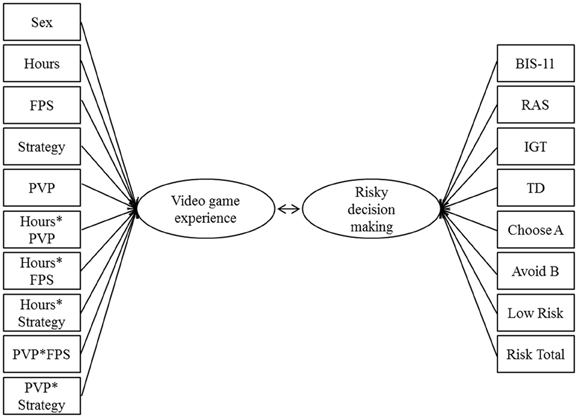
\includegraphics[width=0.8\textwidth]{cca/image/ccafig1.jpg}
    \caption{An example of CCA on behavioural data.}
    \linespacesmall
    \footnotesize
    \caption*{Figure from \citeA{Bailey2013}. Consider a case of exploring the relations between movie genre and personality with CCA. On the left-hand side, we can input the data related to the movies the participants watched, such as the number of action/ documentary/comedy etc. movies watched. The right-hand side is the personality rating of the participants, for example, extrovert vs not, openness vs not etc. The CCA can then find the related personality traits with the type of movies they are likely to watch.}
    \linespacenormal
    \label{fig:methods:fig1}

\end{figure}

\subsection{Joint information compression}
\label{ch:methods:intuitions:1}
 
The purpose of CCA is to find sources of variability that are common to two sets of variables. The relations of a pair of factors across sets of variables, their canonical correlation, indicates the conjoined explained variance across both domains. In a similar manner to PCA, CCA aims to find the most compact linear patterns, canonical variates, based on the variance explained under the contained of uncorrelated hidden dimensions. Also, similar to PCA these dimensions are ranked by their explained variance, with earlier dimensions accounting for more variance than later dimensions. An example of the application of CCA to behavioural data is presented in \cref{fig:methods:fig1}.

\subsection{Symmetry} 
\label{ch:methods:intuitions:2}
CCA does not distinguish between the left and right variable sets during the information compression process. Instead, the canonical correlation indicates that a unit change in a component in one set of observations is consistently associated with an equivalent change in the other set of observations. As CCA does not privilege one of the variable sets, numerically identical decomposition results are returned regardless of the input order of the variable sets. This feature of CCA is known as symmetry and is a key feature that distinguishes CCA from other linear regression methods. The symmetrical nature of CCA can be contrasted with linear-regression models, in which dependent and independent variables play different roles in the analysis. Regression indicates the impact of a unit change in the independent variable on the dependent variables, therefore dependent and independent variables cannot be exchanged to obtain an identical result. As CCA is a correlation-based method, it describes the co-relationship of the two variable sets, thus the exchange of the two variable sets produces identical results.

\subsection{Multiplicity} 
\label{ch:methods:intuitions:3}
In CCA, a pair of dimensions that share variance in both sets of observations is known as a mode. A mode contains a pair of canonical variates that describe the linear structure of the two variable domains. After finding the mode that describes the most variation, CCA will next determine the next pair of dimensions that remains in the unexplained variance of both data sets. Since every new mode was found in the residual variance, the modes are optimised to be uncorrelated with each other. In this manner, CCA produces a set of mutually orthogonal modes naturally ranked by explained variance. The orthogonality constraint ensures the modes represent unique linear patterns that describe different features in the data. When the modes are theoretically meaningful, the researchers can potentially use these to formulate a component process approach to interpret the data.

\subsection{Interim summary}
In conclusion, CCA uncovers effective, symmetric linear relations that compactly summarize doubly-multivariate data. We introduced three important characteristics of CCA. First, CCA provides more effective hidden representation that captures most variance in original variables. Next, the CCA model is symmetrical in the sense that no numerical difference happens in the exchange of the two variable sets. Finally, we can estimate several modes of correspondence between the two variable sets. In the next section, we would like to explore examples of CCA applications.


\begin{figure}[H]
    \centering
    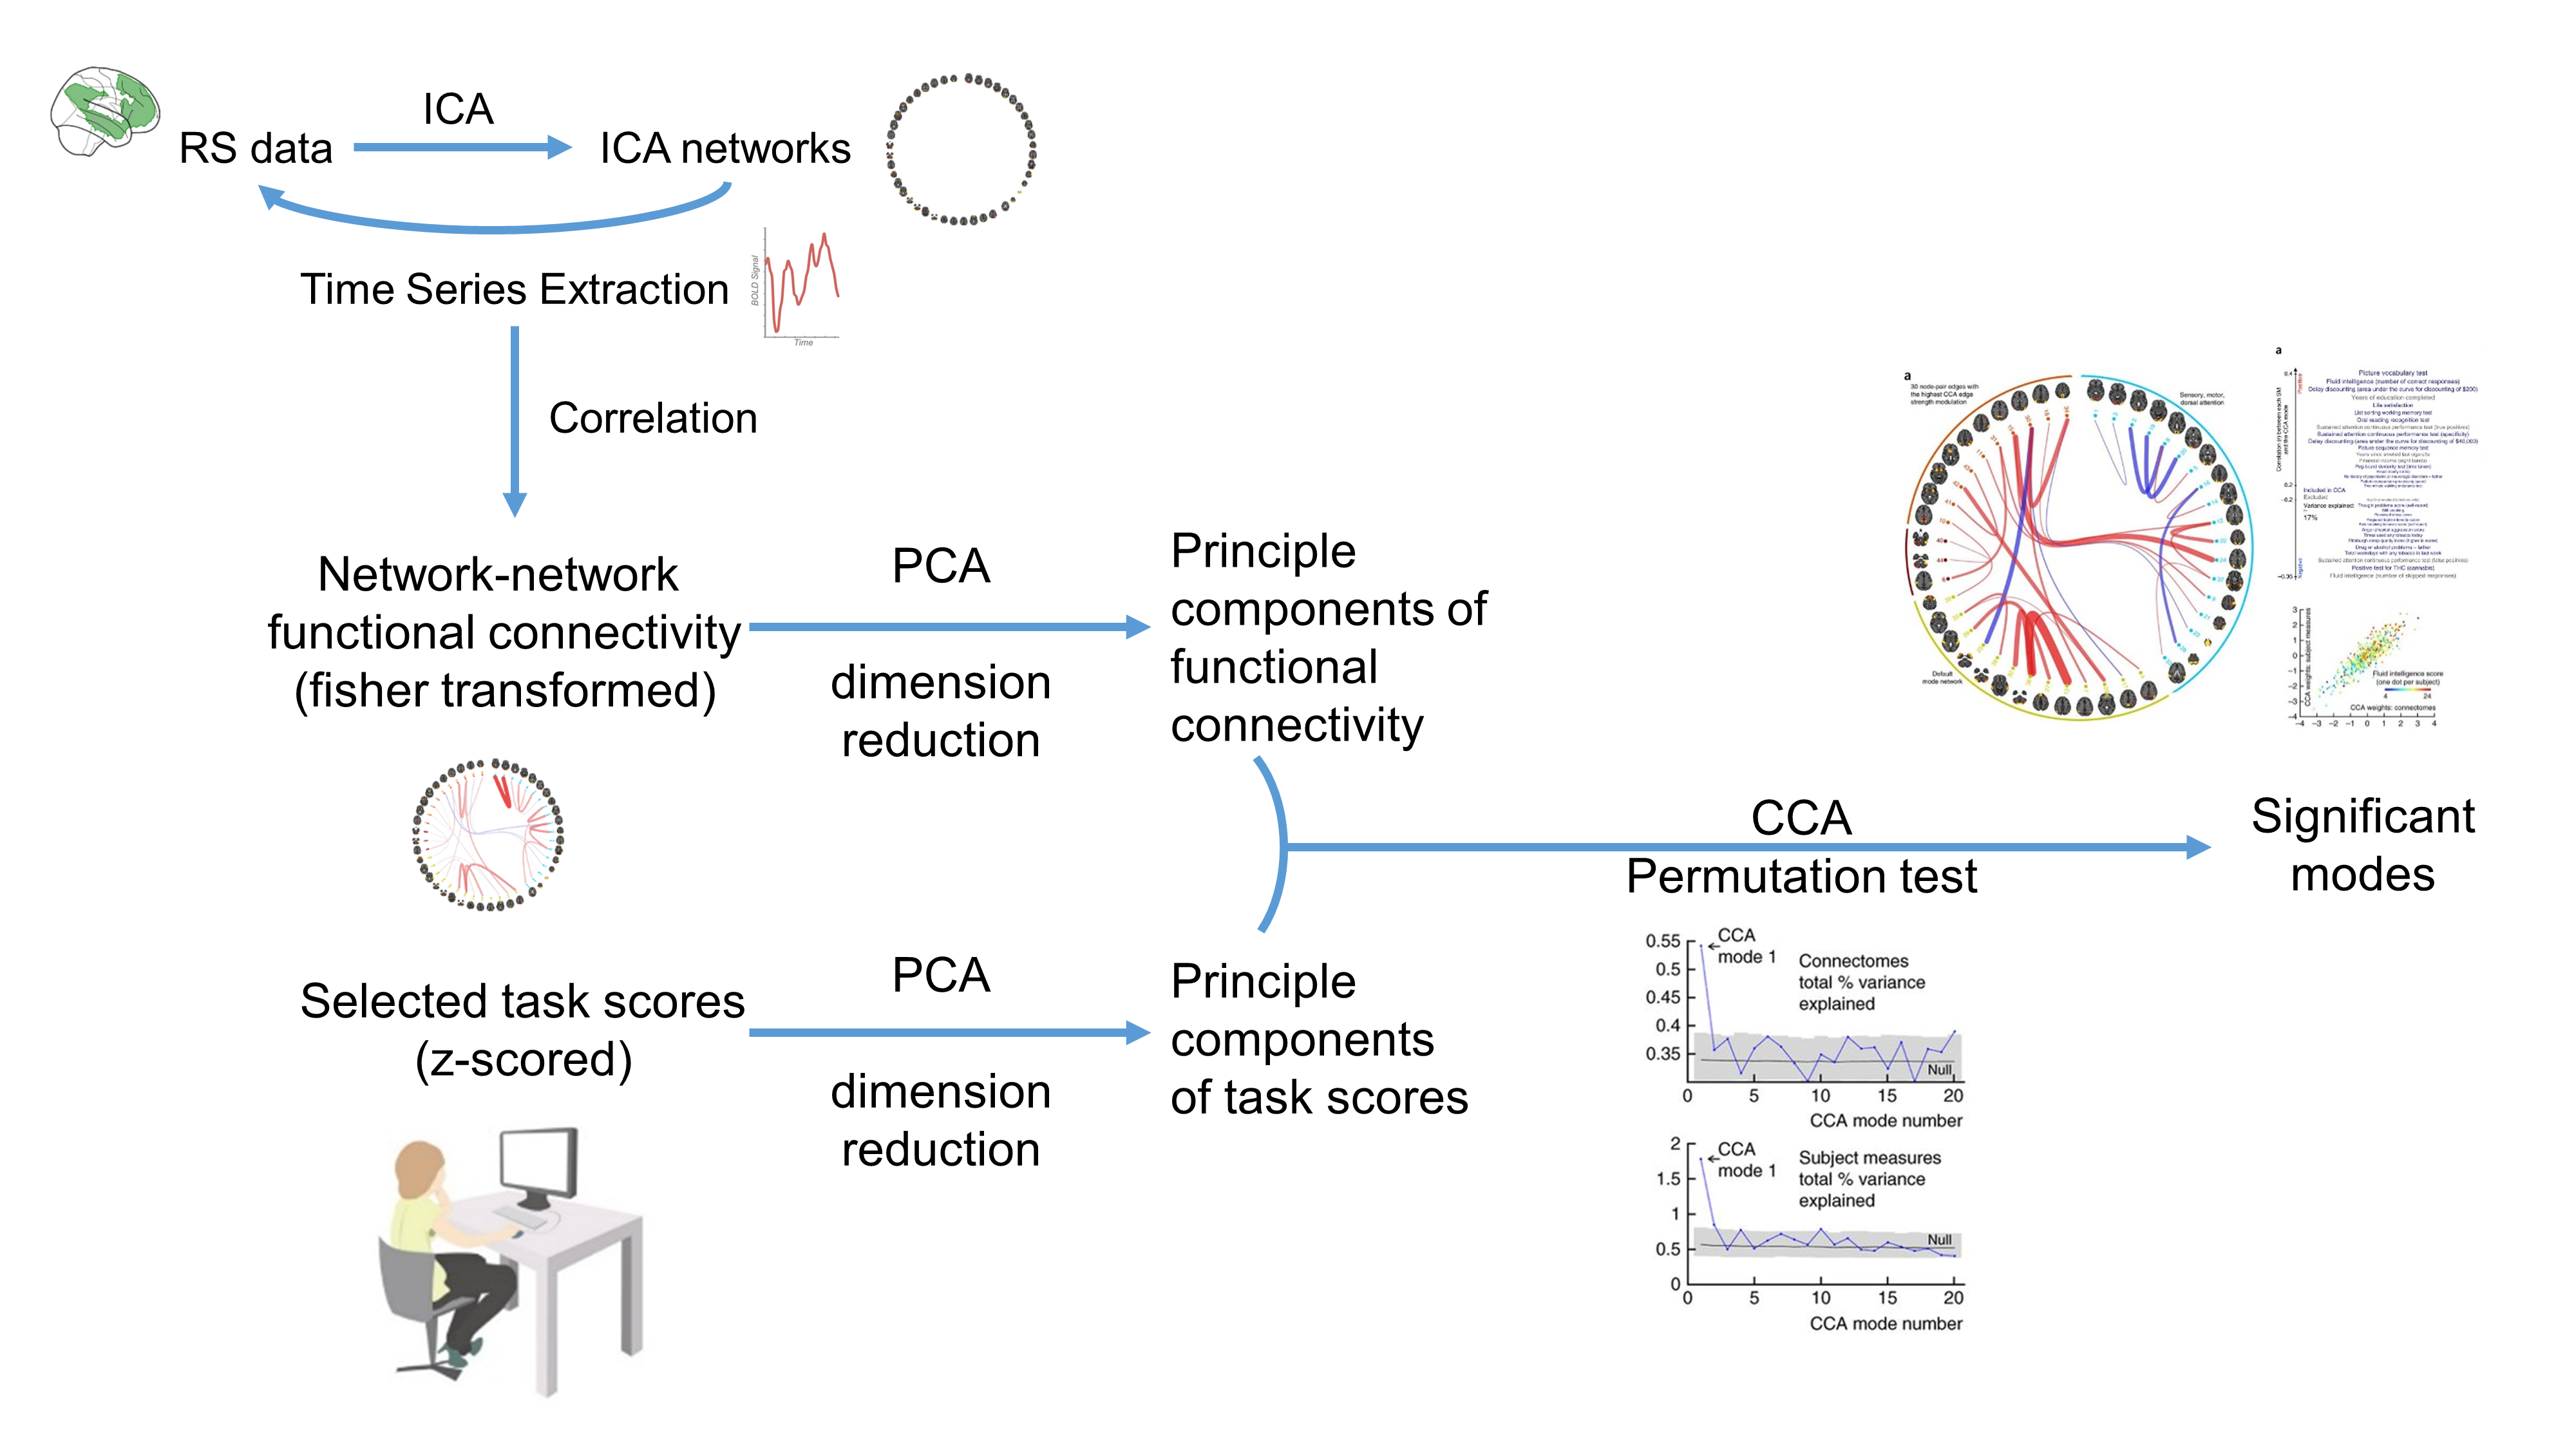
\includegraphics[width=1\textwidth]{cca/image/ccafig2.png}
    \caption{The analysis pipeline of Smith et al. (2015). The arrows represent analysis performed.}

    \label{fig:methods:fig2}
\end{figure}

\section{Examples}

\citeA{Smith2015} employed CCA to uncover brain-behaviour modes of population co-variation in the HCP \cite{VanEssen2013}. \citeA{Smith2015} aimed to discover whether any specific patterns of functional brain connectivity, on the one hand, are associated with specific sets of correlated demographics and behaviour on the other hand (see \cref{fig:methods:fig2} for the analysis pipeline). Functional brain connectivity was retrieved from resting state functional scans which measure the brain activity in the absence of a task or stimulus \cite{Biswal1995}. Independent component analysis \cite<ICA; >{Beckmann2005} was used to identify 200 networks from the resting state scans. ICA identifies independent networks by separating the spatial sources of the resting state data. Next, functional connectivity matrices were calculated based on the pair-wise correlation of the 200 networks. The behavioural measures ranging from cognitive function to demographic information were entered into the CCA as one set of observations and the functional connectivity matrices were the second set. The robustness of the modes was determined via permutation tests on the canonical correlations. One significant mode demonstrated strong population-level co-variation of network connectivity and behavioural measures. The behavioural measures varied along a positive-negative axis with intelligent, memory and cognition tests and life-satisfactory on the positive end and negative lifestyle measures anchoring the other end. The brain regions highly contributing to the connectivity resembles the default mode network \cite<DMN;>{Buckner2008}. The positive-negative dimensions in the behavioural component and the emergence of DMN in the brain component may seem trivial on their own, however, CCA formalised the relation of the underlying biology and the correlation among the general behavioural measures that captures intelligence. Regions composing DMN has been associated with episodic and semantic memory, scene construction, and complex social reasoning such as the theory of mind \cite{Andrews-Hanna2014}. The finding of \citeA{Smith2015} provided evidence that the DMN is important for higher-level cognition, especially intelligence---one of the perhaps most important indices so far identified in by psychologists. 

\begin{figure}[H]
    \centering
    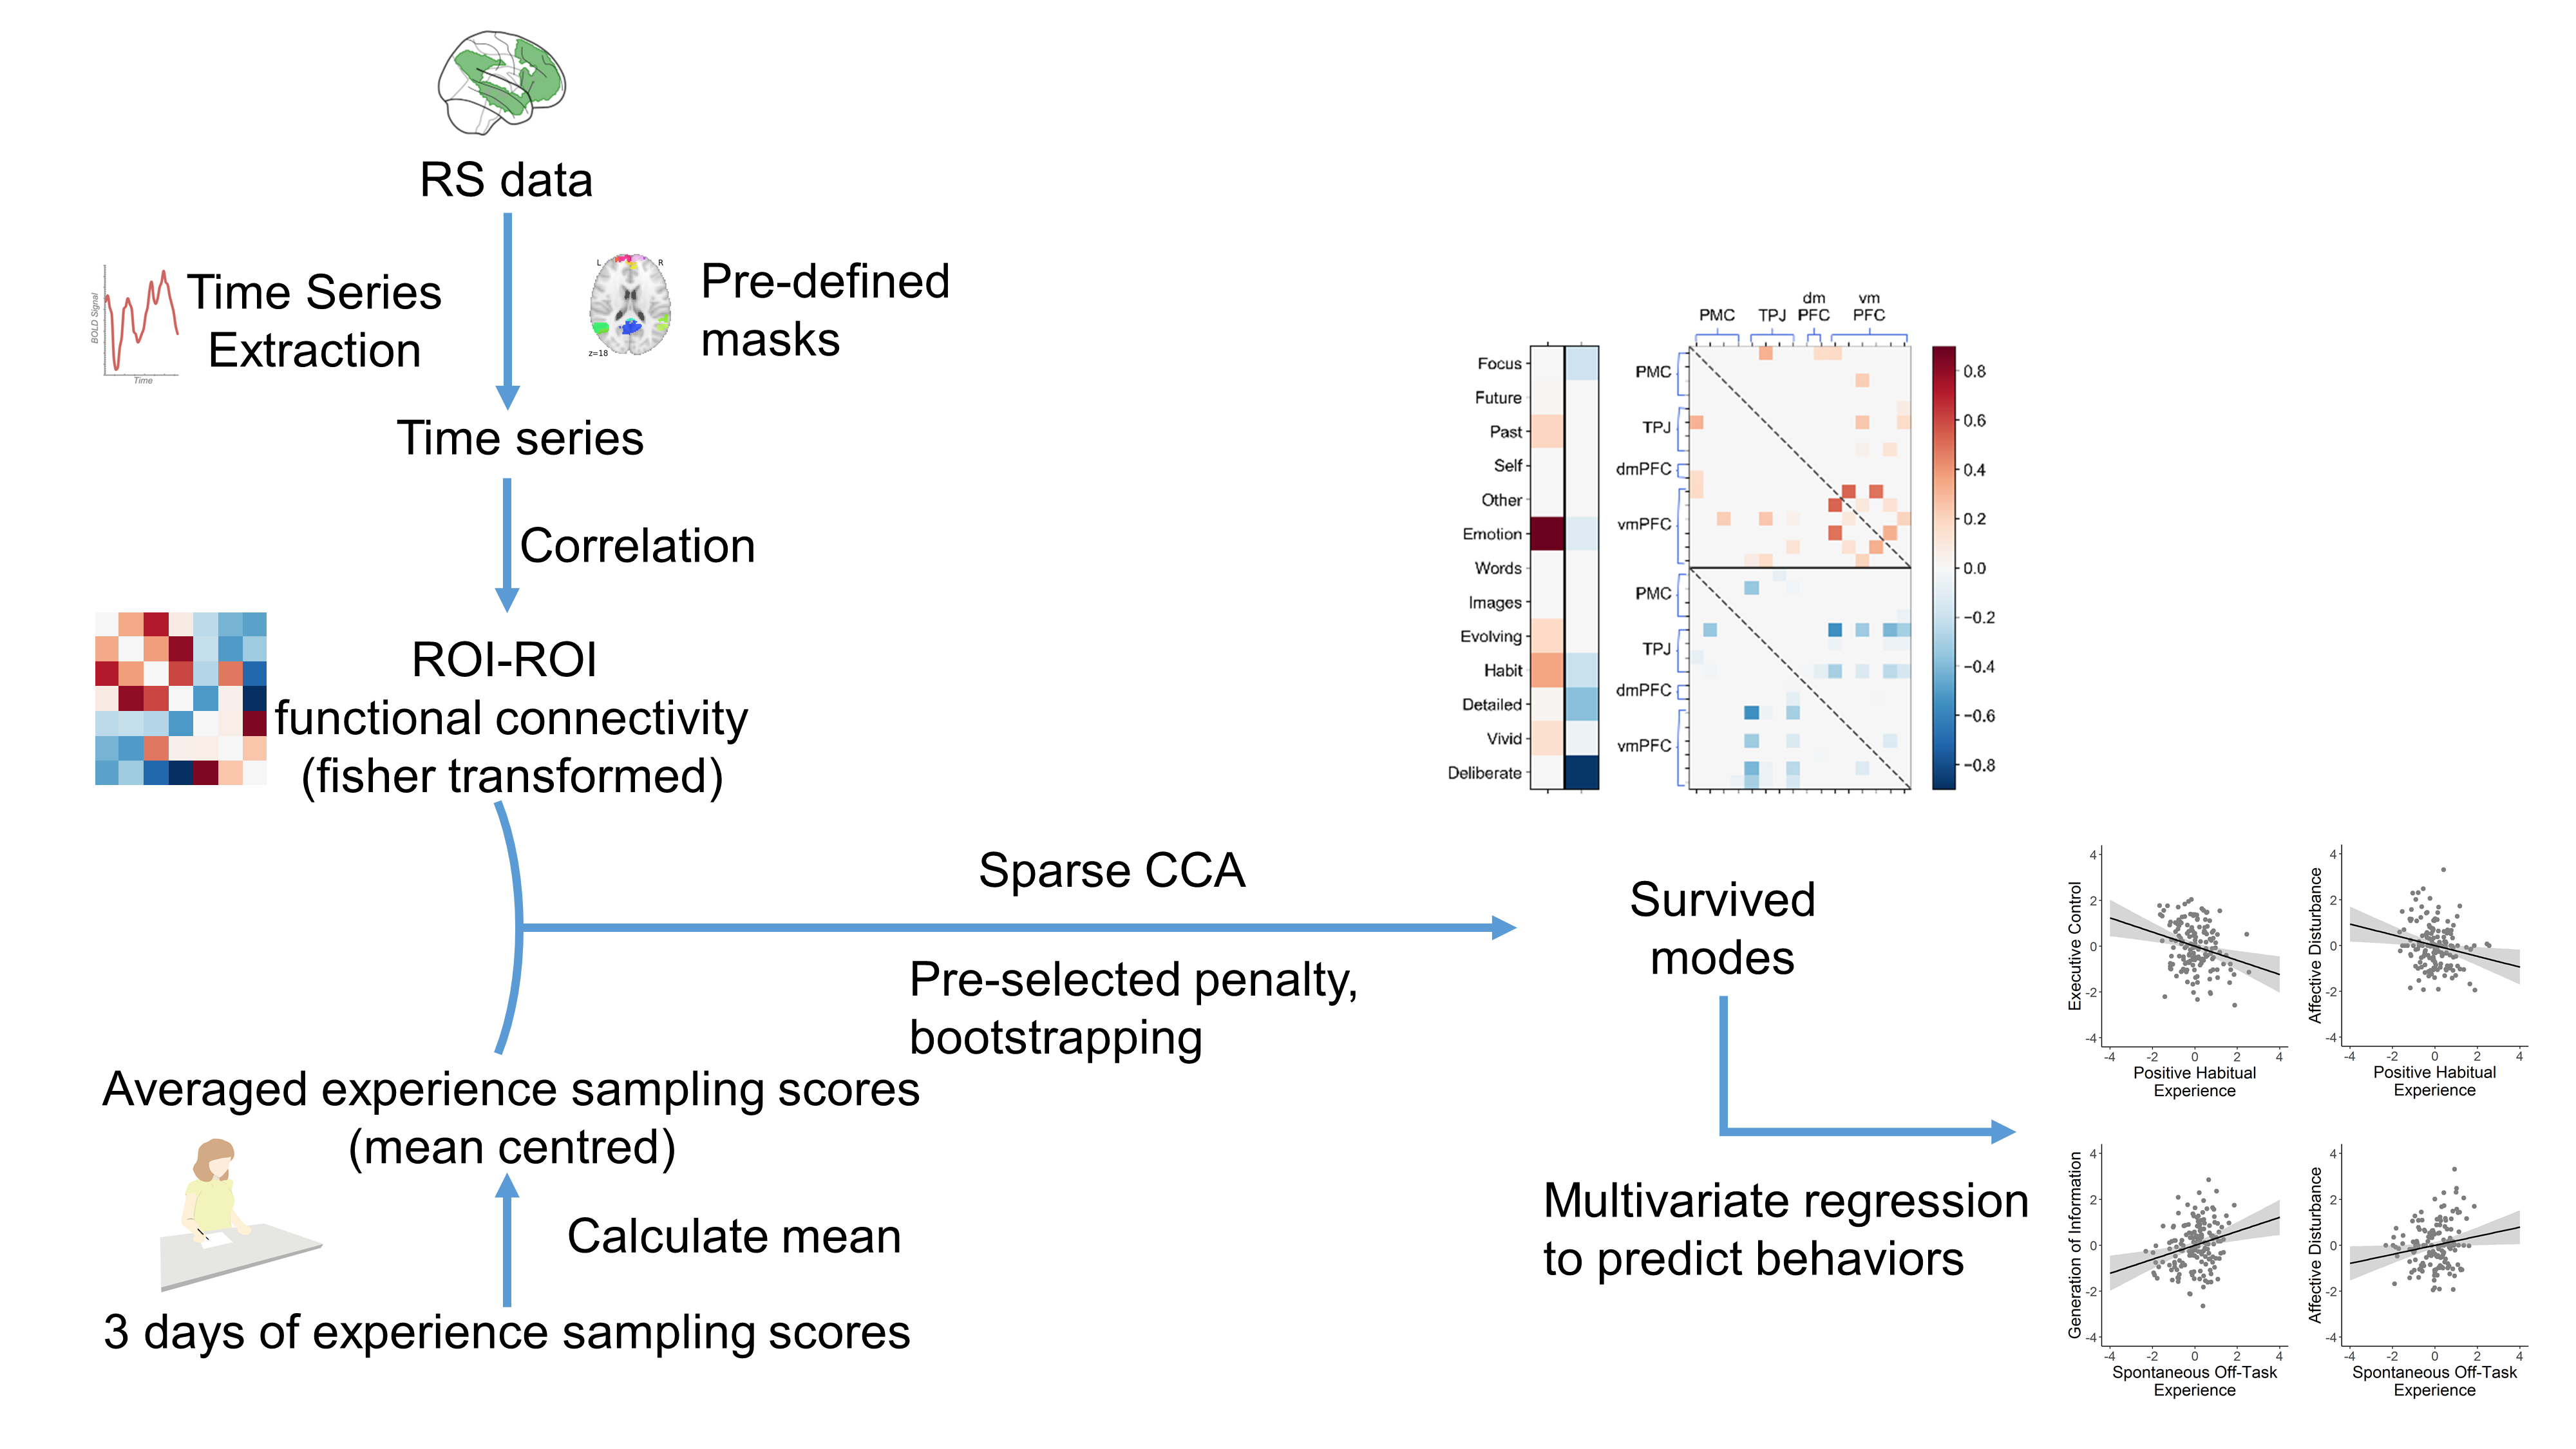
\includegraphics[width=1\textwidth]{cca/image/ccafig3.png}
    \caption{The analysis pipeline of Wang, Poerio et al. (2018). The arrows represent analysis performed.}

    \label{fig:methods:fig3}
\end{figure}
Another use of CCA has been to understand the relationship between patterns of brain activity and variations of experience. \citeA[see \cref{fig:methods:fig3} for the analysis pipeline]{WangPsychScience2018} used CCA to examine links between the DMN and patterns of ongoing thought. In both the laboratory and in daily life, ongoing though can often shift from the task at hand, a phenomenon that is characterised by the experience of mind-wandering \cite{SmallwoodSchooler2006,SmallwoodSchooler2015}. These shifts have been associated with poorer performance on attention-demanding tasks \cite{McVayJOEP2009,MrazekJoEP2012}, yet studies of problem-solving suggest that mind wandering may promote creativity \cite{Baird2012,Smeekens2016} and future planning \cite{Baird2011,Medea2016}. Despite the heterogeneity of functional outcomes, task-unrelated thoughts during mind wandering are linked to changes in DMN activity \cite<see the review from>{SmallwoodSchooler2015}. \citeA{WangPsychScience2018} used CCA to examine the hypothesis that the reason why patterns of off-task thought can have opposing links with behaviour is that there are distinct patterns of the population of variance that link different types of ongoing thought to activity in the DMN. Their analysis used patterns of connectivity within the DMN as one set of observations and self-reported descriptions recorded in the laboratory, recorded across multiple days, as the second set. The connectivity among 16 DMN regions and 13 self-report questions on thoughts were entered using a sparse version of CCA \cite{WittenSCCA2009}. Two stable modes corresponded to traits of positive-habitual thoughts and spontaneous task-unrelated thoughts both with unique patterns of neural connectivity patterns within the DMN. Importantly, subsequent analyses identified that the modes were uniquely related to aspects of cognition, such as executive control and the ability to generate information in a creative fashion, and independently distinguished well-being measures. These data suggest that the DMN can contribute to ongoing thought in multiple ways, each which have unique behavioural associations. \citeA{WangPsychScience2018}, therefore, suggest that mind wandering is a collective term for various types of spontaneous thought \cite<see>{Seli2018}. The different configurations of DMN also demonstrated its possible role as an integrator in cognition, rather than a task-unrelated network \cite{Margulies2016}. 


% ==========================================================================================================


\section{Interpretations}
\label{ch:methods:interpretations}
The symmetrical data compression feature of CCA makes it particularly useful to help researchers handle the complexity of two sets of variables. However, whether the process of the analysis is an exploration of hidden structures or mutually constrained predictive component remains a matter of debate. CCA can be viewed as a supervised predictive algorithm or as an unsupervised exploratory algorithm. A supervised algorithm relies on the predefined labels/relationships in the data to form prediction; whereas an unsupervised algorithm aims to extract patterns in the data with unlabelled data. CCA has some properties of both supervised and unsupervised modelling approach. The more the dimensionality of one of the variable sets resembles the single output of linear-regression-type methods, the more CCA application approaches output are similar to a supervised modelling approach. In contrast, with larger variable sets on both sides, the more CCA resembles an unsupervised modelling approach.

The main difference between supervised and unsupervised method depends on whether there is a set of determined variables as the goal of modelling. To examine whether the model’s prediction matches the desired result, a supervised learning method contains  a learning target or loss function. The difference between the prediction generated by the model and the real label is the objective of a so-called loss function. CCA has as objective to maximise the linear correlation between the latent dimensions from two variable sets. While most supervised learning methods estimate loss between real data and predictions, CCA has an unusual objective that we rarely see in supervised estimators.  Symmetry is another reason that makes CCA an unusual case of supervised learning. In supervised learning, the model learns the pattern in the data to predict a set of targets. The symmetrical nature of CCA does not distinguish the two sets of input variables. The data compression and hidden structure inspection aspect put CCA in line with unsupervised methods. The conjoined decomposition, therefore, captures the relations among the variables. The found relations are used to construct fewer factors that capture the variance of the original data. CCA has the strength of both supervised and unsupervised methods. Like unsupervised methods, CCA can search through candidate patterns to find structure in data. The accurate predictions formed by CCA highlights the trait of a supervised method. In conclusion, CCA is a special case that sits in-between the supervised and unsupervised methods. The flexibility in interpretation offers people multiple ways to utilise CCA in research.

Statistical methods can be categorised into three categories based on their goals: estimation, prediction, and inference.  Estimation represents ways or a process of learning and determining the population parameter based on the model fitted to the data. Prediction is making an inference of an unknown data points based on information obtained from a sample. Inferential statistical analysis utilises hypothesis testing to draw conclusions about populations or scientific truths from data. CCA falls into the family of estimation. The focus of CCA is to establish statistical associations (i.e. the latent linear relations among variables, the association between the two latent linear relations). Predicting some variables based on other variable is not the optimisation goal. CCA does not seek to establish `statistically significant links between variables'. The null hypothesis that is really tested around the robustness of the latent space correlation (i.e., the canonical correlations of the latent variables extracted from the two variable sets) across modes, not so much particular variable-variable links. CCA is often used to rigorously evaluate whether overall linked covariation patterns can be found in two variable sets, rather than pinpointing and `putting the finger on' certain specific relations that should be interpreted with more caution.


% ==========================================================================================================
\subsection{Utility of CCA}
\label{ch:methods:limitations}

CCA does not come without limitations and here we discuss several issues that researchers should keep in mind when evaluating whether the data set is suitable for CCA. We summarise these choices in the form of a flowchart (see \cref{fig:methods:fig4}). As with many statistical approaches, the sample size is an important factor when considering whether CCA is appropriate. CCA can handle data with more observations than the number of variables of the smaller variable set (i.e. \(p< min(m,n)\)). However, smaller data set does not fully utilise the strength of CCA since they tend to have less variability. Relationships in areas like neuroscience are often small, and so a large number of samples is required to correctly infer the variability in data. On the other hand, if the number of variables of either side of the equation exceeds the sample size, CCA does not generate unique linear combinations for each variable set.  In such a scenario, a PCA rank-reduction preprocessing step is commonly performed before applying CCA \cite{Smith2015}. The use of CCA, therefore, is more appropriate when samples sizes are reasonably large relative to the sets of variables being analysed.

\begin{figure}[H]
    \centering
    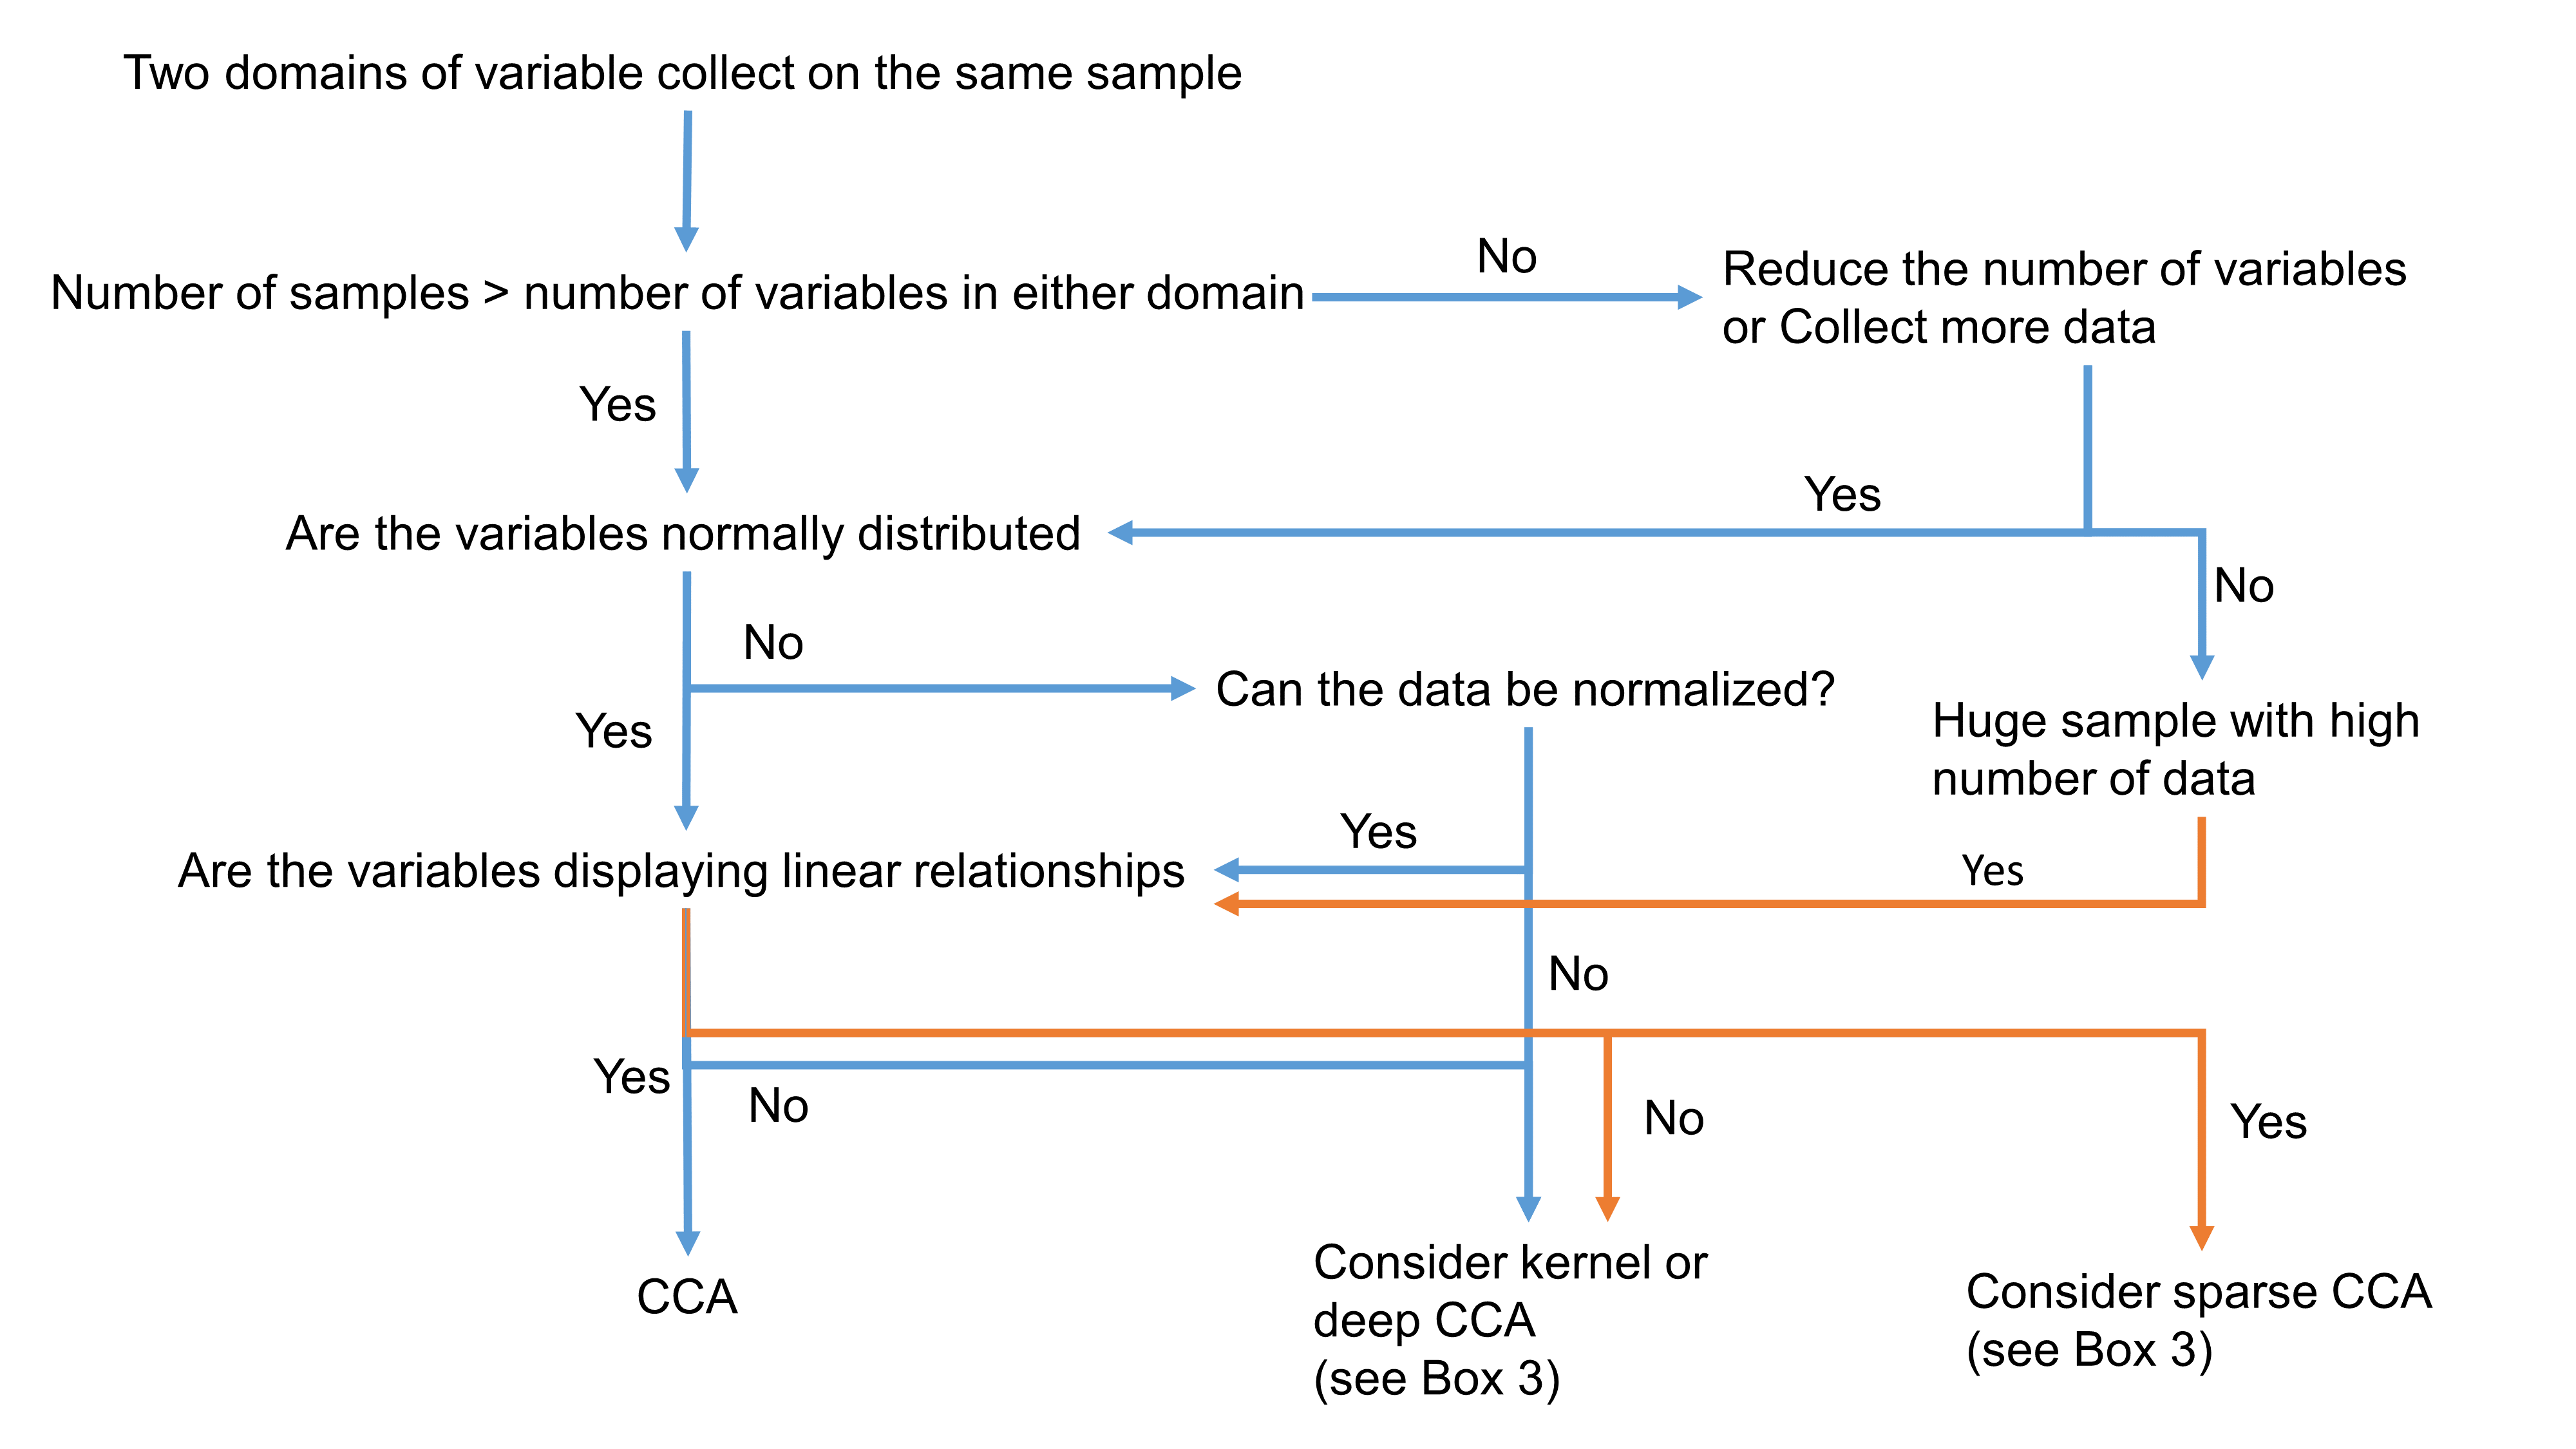
\includegraphics[width=1\textwidth]{cca/image/ccafig4.png}
    \caption{A flowchart illustrating the choices when considering the application of CCA to a dataset.}
    \label{fig:methods:fig4}
\end{figure}

A second issue is the nature of the relationships that CCA describes in the underlying data. CCA is essentially a linear model, and so makes a set of assumptions regarding the normality of the distribution of the observed data, as well as the linearity of the underlying relationships. CCA can accommodate any metric variable without the strict assumption of normality. However, normality is desirable as it allows for the highest correlation among variables, and this makes the task of identifying the underlying dimensions easier. It is recommended to evaluate the normality of all variables and apply data transformation where appropriate before CCA is applied to the data. CCA also assumes that relationships within the data are linear and this introduces two limitations. Since only linear effects can be captured, any patterns within the data that are non-linear (e.g. quadratic or cubic relationships) will not be captured by this analysis. Finally, in CCA relationships are optimised in terms of how effectively they describe linear correlations between variables within the observed data. Relationships discovered by CCA, therefore, should not be considered as predictive accounts of relationships with future data. Any interpretation and application related to predictability of the canonical components in new data should be treated with caution. If the prediction of future observations is important, a small fraction ($20~25\%$) of the full data can be left out as a test data set when the sample size is sufficiently big. The analysis will be applied on the training set first to retrieve the canonical modes. The predictability of the canonical variates from the modes will be examined by calculating the explained variance on the test set.  


\subsection{Relation to other commonly used methods}
CCA can be framed as a general example of other statistical procedures that are derived from the \textbf{general linear model} (GLM). Virtually all of the parametric tests most often used by behavioural scientists (e.g., ANOVA, MANOVA, multiple regression, Pearson correlation, t-test) can be subsumed by CCA as special cases in the GLM \cite{Knapp1978,Thompson2015}. Because these techniques are intricately related and fundamentally the same in many respects of CCA, learning CCA may help facilitate conceptual understanding of statistical methods throughout the GLM.

CCA is related to other feature learning methods in neuroscience. As mentioned in the modelling intuition section, \textbf{PCA} is a similar method performed on one set of variables only. The objective of PCA is a transformation of several possibly correlated variables into a smaller number of uncorrelated variables known as principal components. PCA compresses data into a smaller number of factors that carry most of the variance of the data.

\textbf{Independent component analysis} (ICA) to perform a linear transform that makes the resulting variables as statistically independent from each other as possible. The basic assumption behind ICA is that the data is composed of independent sources of information. In contrast to PCA and CCA, all components are equally important. ICA helps when you want to find a representation of your data as independent sub-elements

\textbf{Partial least squares} (PLS) regression and CCA are both techniques for feature extraction from two sets of multidimensional variables. The fundamental difference between CCA and PLS is that CCA maximizes the correlation while PLS maximizes the covariance. PLS is a supervised approach attempts to find directions that help explain both the response and the predictors. Most of the comparison between PLS and CCA is focused on the generation of the first components. There is no one way to compute the other components in PLS \cite{DeBie2005}.

Several useful extensions of CCA has emerged in the past decade to overcome the limitation of the linear version of CCA. The first was the nonlinear version of CCA, with \textbf{kernelization of CCA} \cite<KCCA;>{Hardoon2004} as the representative.  Kernels are methods of implicitly mapping data into a higher-dimensional feature space with kernel function, a method known as the kernel trick. KCCA first project the data into a higher-dimensional feature space before performing CCA in the new feature space.  While KCCA allows learning of nonlinear representations, the drawback is that the representation is limited by the fixed kernel. KCCA is a nonparametric method, hence, the time required to train KCCA or compute the representations of new data points scales poorly with the size of the training set.

\textbf{Sparse CCA} \cite<SCCA;>{WittenSCCA2009} is a method for identifying sparse linear combinations of the two sets of variables that are highly correlated with each other. It has been shown to be useful in the analysis of high-dimensional data when the variable number of either array is higher than the number of samples. The sparse feature reduces some coefficients to 0 in the linear structure depending on the penalty parameters. The benefit of sparsity is an improvement in interpretation and feature selection. However, sparsity violates the orthogonality of CCA, meaning the components in different modes can correlate with each other. The explained variance of each mode will not follow the rank order either. Recently, we have used k-fold cross-validation to identify the ideal level of sparsity in a study that explores the relationship between patterns of thought at rest and the associated brain organization \cite{WangNI2018}.

With the recent advance in the deep neural network, \textbf{deep CCA} \cite<DCCA;>{AndrewDCCA2013} has been proposed as an alternative to KCCA as a non-linear method for CCA. A deep neural network is an algorithm that learns the representation of data through multiple non-linear transformations. The name came from the architecture that loosely follows the connections of neurons. DCCA simultaneously learns two deep neural network mappings of two variable sets that are maximally correlated. The main advantage is the faster performance over KCCA because DCCA directly learns the data without re-mapping data into a higher dimension. 

% ==========================================================================================================


\section{Practical considerations}
\label{ch:methods:impliment}

Having introduced the features and interpretations of CCA, we close by considering the practical considerations that determine how it should be implemented. The computation of CCA is available in the in-built library of MATLAB (\texttt{canocorr}) and R (\texttt{cancor}), and Python machine-learning library scikit-learn (\texttt{sklearn.cross\_decomposition.CCA}). All implementations above provides comprehensive documentation for how to implement CCA and we describe the additional steps that a researcher may wish to consider before applying CCA to their data.

\subsection{Preprocessing}
Some minimal data preprocessing is usually required for most machine-learning methods. The objective of CCA is maximising correlations between two input variable sets. The nature of correlation is defined by the degree of simultaneous unit change between two variables; therefore, the computational process has implicitly standardised the data and the features obtained from CCA are scale invariant (cf. PLS optimises the covariance; therefore, the output will be influence by scaling.). \textbf{Scaling}, such as z-scoring, is still recommended before performing CCA for the ease of interpretation. This helps people to focus on unit chance rather than absolute values of data. The linear relationship is also sensitive to outlier effects. To avoid outliers skewing the results, application of \textbf{outlier detection techniques} and \textbf{outlier cleaning} are recommended before the analysis, such as imputation with the mean or median of the variables. Aside from outliers, some confound variables can also introduce unwanted effects. Confound variable removal is recommended as a preprocessing step to reduce the risk of finding non-meaningful associations. The same rules are also commonly applied for the GLM in the neuroimaging data. The subsequent analysis would reflect the data without influences of the confound. In neuroimaging, for example, motion is thought to be an important confound \cite{Power2014} and as consequence, it is common to remove the influence of this variable prior to conducting CCA \cite<see>{WangNI2018}.

When the number of variables exceeds the number of samples, PCA is recommended as a preliminary \textbf{dimension reduction} step before performing CCA. An example is work by  \citeA{Smith2015}. The application of PCA compresses the number of variables in each matrix to the most explanatory dimension of variation. However, a  downside of this method is the difficulty to directly map the resulting dimensions to the original data. To interpret the CCA solutions in the original data, \citeA{Smith2015} correlate the canonical variates to the original data to recover the relevant variate captured by the CCA component pair.  

CCA component can be challenging to interpret, especially when a PCA dimension reduction is applied. An alternative solution is a \textbf{CCA+ICA} method in addition to the PCA \cite{MillerK2016,Sui2010} has been proposed to overcome the issue of projecting the PCA-compressed data back to the original space. In the original CCA+ICA approach, the assumption is that CCA extracted components are an incomplete decomposition with multiple possible sources (i.e. patients vs controls). CCA first finds the correlated variance of the two variable set. After CCA, the canonical components are concatenated into one array. ICA is then applied to the canonical components to recover the source of the variance. The ICA step can be done in the full feature space by projecting the CCA components to the PCA components \cite{MillerK2016}. The CCA+ICA approach achieves both high estimation accuracy and to provide the correct connection between two variable sets. The ICA step is especially useful in the detection of independent components that contribute to the common solution extracted from the two variable sets.

\subsection{Model selection}
CCA allows multiple modes to be calculated from the observed data, however, it is necessary to specify the appropriate number of these latent sources of variation. To select the number of modes (canonical component pair, see \cref{ch:methods:intuitions}), we can use \textbf{explained variance} metrics to determine a useful number of modes. Since the canonical components are the compressed information of the original data, the canonical component would be expected to be related to the original data. The calculation can be done by predicting the canonical components with the original scores. Another solution is to calculate the family-wise error rate through \textbf{permutation tests}. The incentive of permutation test is to access the robustness of results when comparing to results from randomly re-arranged data. The permutation is done on randomising one of the variable sets to break the unique relationship between the two variable sets in each observation instance. The extracted modes from the randomised sample will serve as the chance level results. Permutation tests establish robust above-chance correspondences between variable sets, but no null hypothesis significance testing for an individual variable is tested this way. The first canonical correlation of the permuted sample is compared with all the CCA modes extracted from the real data . The p-value for each mode is calculated as the number of permuted sample canonical correlation higher than the given mode from the real sample, divided by the number of permutation.

The variations of CCA might need an extra step for \textbf{hyperparameters selection}, such as the knobs of kernel type and penalty in KCCA, penalty strengths in SCCA, and layer number in DCCA. A permutation or cross-validation scheme is recommended for hyperparameters selection. The permutation test on hyperparameter selection is set up in the same way as model selection, but focusing on the first canonical correlation only\cite<For example, see Appendix A in>{WittenSCCA2009}. In terms of cross-validation, the objective function for model selection can be the out-of-sample explained variance or the variance loss between the training set and the testing set. 

% ==========================================================================================================
\section{Summary}
\label{ch:methods:summary}
In biomedicine research, the relationships among brain, cognition and disease are often complicated. Focusing on a small selection of measures will risk in ignoring potential factors. CCA is a doubly multivariate pattern analysis on two variable sets.  With no directionality implied on either variable set, CCA enables more flexibility on the research questions. As the interest in multitask data and rich cognitive phenotyping in large dataset grows, CCA fulfills the need of a method that can considers a large set of possible variables in one analysis. With its ability to reduce the data to meaningful and concise information, CCA is a promising method for scientists who are interested in exploration of multivariate patterns in large data sets.